\documentclass[12pt, twoside]{article}
\usepackage[francais]{babel}
\usepackage[T1]{fontenc}
\usepackage[latin1]{inputenc}
\usepackage[left=1cm, right=1cm, top=1cm, bottom=1cm]{geometry}
\usepackage{float}
\usepackage{graphicx}
\usepackage{array}
\usepackage{multirow}
\usepackage{amsmath,amssymb,mathrsfs}
\usepackage{textcomp}
\usepackage{soul}
\pagestyle{empty}
\begin{document} 

\textbf{Exercice 4:}

\begin{enumerate}
  
  \item Construire une droite $(d)$ et placer deux points $A$ et $B$ qui
  n'appartiennent pas � la droite $(d)$.
  \item Construire en rouge la droite $(d_{1})$ perpendiculaire � $(d)$ passant
  par $A$.
  \item Construire en vert la droite $(d_{2})$ perpendiculaire � $(d)$ passant
  par $B$.
  \item  Que peut-on dire des droites $(d_{1})$ et $(d_{2})$?
  \item Recopier et compl�ter la phrase: \textit{Les droites $(d_{1})$ et
  $(d_{2})$ sont \ldots \ldots \ldots \ldots \ldots parce qu'elles sont toutes les deux
  \ldots\ldots\ldots\ldots\ldots\ldots � la droite (\ldots).}
  \item Citer la propri�t� du cours qui permet de l'affirmer?
 \item Recopier et compl�ter:
 \begin{center}
 
\begin{tabular}{cc}
 \begin{minipage}{6cm}
 \ul{Donn�es}\\
 \ldots \ldots \ldots \ldots \ldots\\
 \ldots \ldots \ldots \ldots \ldots
 \end{minipage}       
&  
\begin{minipage}{6cm}
\ul{Conclusion}
\medskip

donc \ldots \ldots \ldots \ldots
\end{minipage}
 \end{tabular}
  \end{center}
  \end{enumerate}

\bigskip

\textbf{Exercice 5:}


\bigskip

\begin{tabular}{cc}
\begin{minipage}{9cm}

\includegraphics[width=6cm]{images/ex4.png}
\end{minipage}
&
\begin{minipage}{9cm}
Compl�ter le texte suivant:


On sait que les droites \ldots \ldots et \ldots \ldots sont \ldots \ldots \ldots
\ldots \ldots.

 Or si deux droites sont perpendiculaires � une m�me droite alors
elles sont \ldots \ldots \ldots \ldots \ldots entre elles. 

Donc on a:  \ldots \ldots et \ldots \ldots
sont parall�les.
\end{minipage}
\end{tabular}

\bigskip 

\textbf{Exercice 6:}

\begin{enumerate}
  
  \item Construire une droite $(d)$ et placer deux points $A$ et $B$ qui
  n'appartiennent pas � la droite $(d)$.
  \item Construire en rouge la droite $(d_{1})$ parall�le � $(d)$ passant
  par $A$.
  \item Construire en vert la droite $(d_{2})$ perpendiculaire � $(d)$ passant
  par $B$.
  \item  Que peut-on dire des droites $(d_{1})$ et $(d_{2})$?
  \item Recopier et compl�ter la phrase: \textit{Les droites $(d_{1})$ et
  $(d_{2})$ sont \ldots \ldots \ldots \ldots \ldots parce que les
  droites (\ldots) et (\ldots) sont perpendiculaires et les droites (\ldots) et
  (\ldots) sont parall�les entre elles.}
  \item Citer la propri�t� du cours qui permet de l'affirmer?
 \item Recopier et compl�ter:
 \begin{center}
 
\begin{tabular}{cc}
 \begin{minipage}{6cm}
 \ul{Donn�es}\\
 \ldots \ldots \ldots \ldots \ldots\\
 \ldots \ldots \ldots \ldots \ldots
 \end{minipage}       
&  
\begin{minipage}{6cm}
\ul{Conclusion}
\medskip

donc \ldots \ldots \ldots \ldots
\end{minipage}
 \end{tabular}
  \end{center}
  \end{enumerate}

\bigskip

\textbf{Exercice 7:}


\bigskip

\begin{tabular}{cc}
\begin{minipage}{9cm}
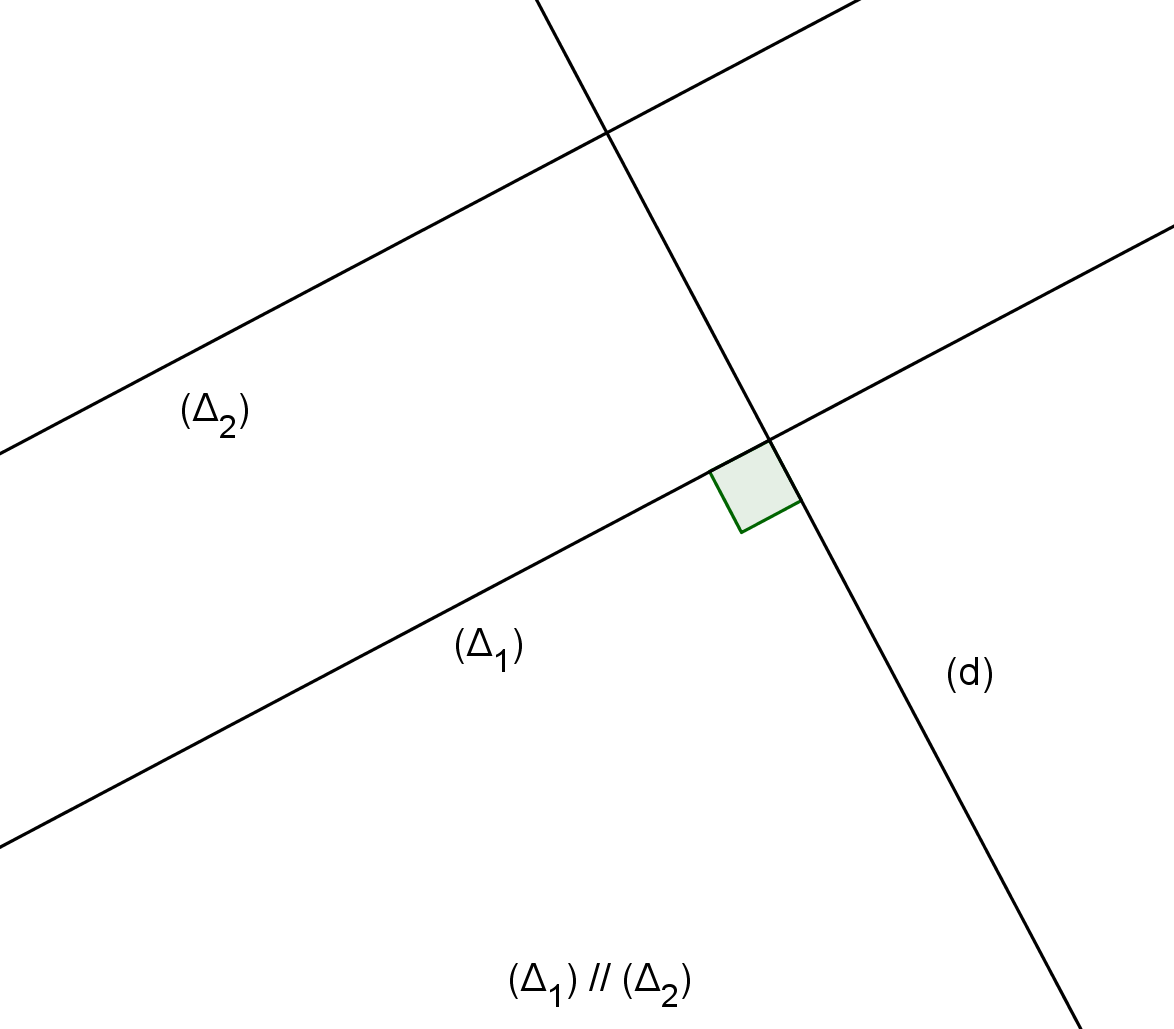
\includegraphics[width=7cm]{images/ex7.png}
\end{minipage}
&
\begin{minipage}{9cm}
Compl�ter le texte suivant:


On sait que les droites \ldots \ldots et \ldots \ldots sont perpendiculaires.
On sait aussi que les droites ($\Delta_{1}$) et ($\Delta_{2}$) sont
\ldots \ldots \ldots \ldots \ldots.


 Or si deux droites sont parall�les alors toutes droites perpendiculaires 
� l'une est \ldots \ldots \ldots \ldots \ldots \ldots � l'autre.

Donc on a:  \ldots \ldots et \ldots \ldots
sont perpendiculaires. 
\end{minipage}
\end{tabular}

\bigskip 

\end{document}
